\documentclass{article}
\usepackage{graphicx} % Required for inserting images
\usepackage{booktabs}
\usepackage{array}

\title{Relat\'orio A2 -- DijkFood\\Computa\c{c}\~ao em Nuvem}
\author{Elisa Soares \and Maria Eduarda Mesquita \and Mariana Fernandes \and Raphaella Roma}
\date{June 2026}

\begin{document}

\maketitle

\section{Arquitetura}

\begin{figure}[h]
\centering
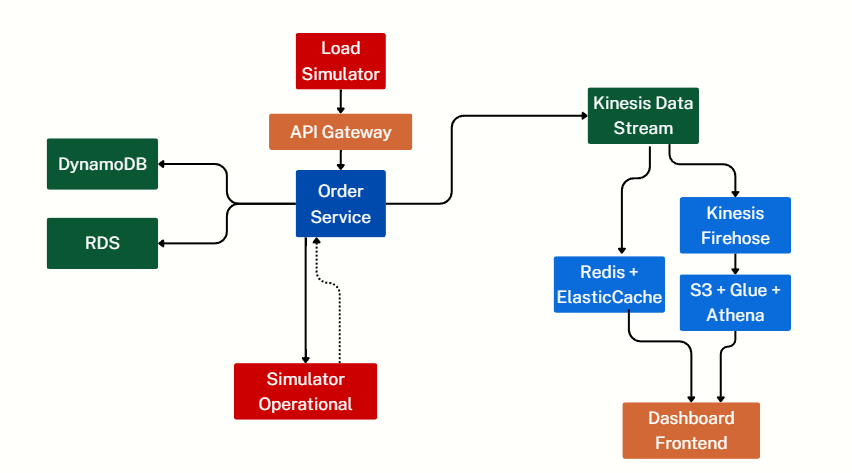
\includegraphics[width=\textwidth]{arquitetura-final.png}
\caption{Arquitetura geral do DijkFood}
\label{fig:arquitetura}
\end{figure}

O fluxo come\c{c}a no \textbf{Load Simulator}, respons\'avel por gerar carga sint\'etica para o sistema. Ele envia requisi\c{c}\~oes para a API por meio do \textbf{API Gateway}, que representa o ponto de entrada do sistema. A partir desse ponto, as chamadas chegam ao \textbf{Order Service}, servi\c{c}o central da aplica\c{c}\~ao. Esse servi\c{c}o coordena a cria\c{c}\~ao dos pedidos, consulta e atualiza dados persistentes e publica eventos de mudan\c{c}a de estado.

Na camada de persist\^encia, o sistema utiliza dois tipos de armazenamento. O \textbf{RDS} armazena dados relacionais da aplica\c{c}\~ao, como pedidos, usu\'arios, restaurantes e entidades transacionais. O \textbf{DynamoDB} \'e usado para dados que se beneficiam de acesso r\'apido e escalabilidade horizontal, como localiza\c{c}\~ao ou estado operacional de entregadores. Essa separa\c{c}\~ao permite usar banco relacional onde h\'a relacionamento forte entre entidades e banco NoSQL onde h\'a necessidade de baixa lat\^encia e alto volume de leitura/escrita.

O \textbf{Simulador Operacional} representa o comportamento externo do ambiente de delivery. Ele simula etapas como aceita\c{c}\~ao do pedido, preparo, despacho e entrega. Na arquitetura, ele se comunica com o Order Service para gerar mudan\c{c}as de estado e alimentar o ciclo de vida dos pedidos. Assim, o sistema consegue produzir eventos semelhantes aos de uma opera\c{c}\~ao real, mesmo sem usu\'arios humanos interagindo continuamente.

Sempre que eventos relevantes ocorrem, o Order Service publica registros no \textbf{Kinesis Data Stream}. Esse componente funciona como a espinha dorsal de eventos da arquitetura. Ele desacopla a gera\c{c}\~ao dos eventos do consumo posterior, permitindo que diferentes consumidores leiam o mesmo fluxo de dados sem depender diretamente do Order Service.

A partir do Kinesis, existem dois caminhos principais de observa\c{c}\~ao. O primeiro \'e o caminho de \textbf{tempo real}, no qual os eventos s\~ao consumidos por servi\c{c}os de m\'etricas e podem ser propagados para o \textbf{Redis/ElastiCache}. No ambiente local, esse componente \'e um Redis em container; na AWS, ele \'e representado pelo \textbf{Amazon ElastiCache for Redis}. Ele pode atuar tanto como banco de snapshots quanto como mecanismo de Pub/Sub, permitindo que o dashboard receba atualiza\c{c}\~oes com baixa lat\^encia, mas aqui, como fluxo final decidimos por pub-sub (o que será defendido em uma seção posterior).

O segundo caminho \'e o caminho \textbf{anal\'itico}. Nele, os eventos do Kinesis s\~ao enviados para o \textbf{Kinesis Firehose}, que grava os dados no \textbf{S3}. Em seguida, o \textbf{Glue} organiza o cat\'alogo dos dados e o \textbf{Athena} permite consultas SQL sobre os eventos armazenados. Esse fluxo n\~ao tem como objetivo atualizar a interface em tempo real, mas sim permitir an\'alises hist\'oricas, agrega\c{c}\~oes por per\'iodo e relat\'orios posteriores.

Por fim, o \textbf{Dashboard Frontend} consome tanto os dados de tempo real quanto os dados anal\'iticos. Para a vis\~ao operacional, ele recebe snapshots via WebSocket a partir dos servi\c{c}os de m\'etricas e do Redis/ElastiCache. Para a vis\~ao hist\'orica, ele consulta resultados agregados vindos da trilha S3, Glue e Athena. Dessa forma, a arquitetura separa claramente o que precisa de baixa lat\^encia do que pode ser processado de forma ass\'incrona e anal\'itica.

\section{Gargalos}

\subsection{Gargalo no Routing Service}

Durante o desenvolvimento, a integração do \textit{courier-simulator} com o \textit{routing-service} introduziu um gargalo não imediatamente óbvio. Após a correção da rota do entregador, que passou a seguir o caminho calculado pelo algoritmo de Dijkstra em vez de uma interpolação direta entre dois pontos, o sistema apresentou um comportamento indesejado: havia muitos pedidos no estado \textit{ready to pickup} e entregadores disponíveis, mas apenas um ou dois entregadores processavam entregas simultaneamente.

A causa foi identificada na forma como o \textit{delivery-service} solicitava rotas ao \textit{routing-service}: todas as requisições eram processadas por uma única \textit{task}, criando uma fila serializada. Os entregadores existiam e estavam disponíveis, mas ficavam bloqueados aguardando a resposta de rota antes de iniciar o deslocamento. O gargalo não estava na alocação nem na quantidade de entregadores, mas na capacidade de processamento paralelo das requisições de roteamento.

A solução foi o aumento do número de \textit{tasks} paralelas dedicadas ao \textit{routing-service}, permitindo que múltiplas requisições de rota fossem processadas simultaneamente. Adicionalmente, o serviço foi colocado atrás de um balanceador de carga, permitindo distribuir as requisiçõoes entre múltiplas instâncias, e o \textit{autoscaling} foi reconfigurado com base no volume de \textit{requests}. Com isso, a capacidade do \textit{routing-service} passa a crescer conforme a demanda observada, reduzindo o risco de ele se tornar o ponto único de contenção no fluxo de entregas.

\section{Dashboard}
\subsection{Fluxo em tempo real}

A origem comum dos quatro caminhos é o \textit{Kinesis Data Stream}, que recebe eventos do ciclo de vida dos pedidos, como criação, mudança de status, atribuição de entregador e conclusão da entrega. A partir desse ponto, os caminhos são independentes entre si: cada um consome ou propaga os dados de uma forma diferente e publica snapshots para o dashboard por WebSocket.

O primeiro caminho é o \textbf{Realtime Metrics Service sem PySpark}. Nesse fluxo, o serviço FastAPI possui um consumidor direto do Kinesis implementado com \texttt{boto3}. O consumidor percorre os shards do stream, desserializa cada registro, identifica o formato do evento e atualiza um estado agregado em memória. Esse estado mantém contadores de pedidos em preparo, aguardando entregador, em entrega, entregues, entregadores disponíveis e latências de ingestão. A cada segundo, o backend envia o snapshot diretamente ao dashboard por WebSocket. Esse caminho tem a menor complexidade operacional, pois não depende de uma camada intermediária além do próprio serviço de métricas.

O segundo caminho usa \textbf{Redis como banco de snapshots}. Um worker separado também consome o Kinesis em paralelo, calcula as mesmas métricas agregadas e grava o resultado no Redis com uma chave de snapshot e tempo de expiração. O backend do dashboard consulta periodicamente esse snapshot no Redis e repassa o conteúdo para o navegador por WebSocket. Nesse desenho, o Redis funciona como uma camada de estado compartilhado: ele desacopla o cálculo das métricas da entrega para o dashboard e permite que múltiplas instâncias do backend leiam o mesmo snapshot. A desvantagem é que existe uma etapa extra de escrita e leitura, o que tende a adicionar latência e a exigir cuidado com TTL, consistência do snapshot e frequência de atualização.

O terceiro caminho usa \textbf{Redis como Pub/Sub}. Nesse fluxo, o worker que consome o Kinesis não apenas grava o snapshot no Redis, mas também publica a mensagem em um canal Redis Pub/Sub. O backend do dashboard fica inscrito nesse canal e, ao receber cada publicação, encaminha o snapshot imediatamente para os clientes WebSocket. A principal diferença em relação ao Redis como banco é o padrão de comunicação: em vez de consultar uma chave periodicamente, o backend recebe uma notificação por push. Isso reduz o custo de polling e tende a ser melhor para baixa latência, embora mensagens Pub/Sub sejam efêmeras: se um consumidor estiver desconectado, ele não recebe publicações antigas.

O quarto caminho usa \textbf{PySpark para métricas em tempo real}. Esse pipeline também consome eventos do Kinesis, mas processa uma janela recente de eventos usando uma sessão PySpark local. O objetivo é avaliar se uma ferramenta de processamento distribuído traria vantagem para agregações mais pesadas. Nesse caso, os eventos são convertidos para estruturas compatíveis com Spark, agregados por janela e transformados em snapshots enviados ao dashboard. A vantagem desse caminho aparece quando o volume de dados e a complexidade das transformações justificam um motor distribuído. Entretanto, para o dashboard operacional existe um custo adicional de inicialização, serialização e execução do Spark, o que pode impactar o desempenho em cargas maiores.

Para comparar os caminhos, foi executada uma carga local controlada com 5 pedidos por segundo durante 60 segundos, totalizando 300 tentativas de pedido. O sistema aceitou 246 pedidos e concluiu 71 entregas durante a execução observada. A métrica principal da comparação foi \texttt{event\_to\_dashboard\_emit\_latency\_ms}, que mede o intervalo entre o timestamp do evento original e o momento em que o backend emite o snapshot para o dashboard. Portanto, os valores refletem o tempo fim a fim entre o evento publicado no fluxo e a emissão da atualização visual, e não apenas o tempo de processamento interno de cada componente.

Nas tabelas, a coluna \textbf{amostras} representa a quantidade de medições de latência coletadas para cada caminho a partir dos snapshots emitidos pelo backend; ela não representa diretamente a quantidade de pedidos criados. A coluna \textbf{média} representa a latência média dessas amostras. A coluna \textbf{p50} representa o percentil 50, ou seja, metade das medições teve latência menor ou igual àquele valor. A coluna \textbf{p95} representa o percentil 95, isto é, 95% das medições ficaram abaixo daquele valor. Em sistemas de tempo real, o p95 é importante porque mostra o comportamento da cauda da distribuição, indicando se uma parte dos usuários recebe atualizações muito atrasadas mesmo quando a média parece aceitável.

A Tabela 1 mostra o comportamento em um cenário controlado. Nesse cenário, o caminho com \textbf{PySpark} apresentou os melhores resultados absolutos, com menor média, menor p50 e menor p95 entre todos os caminhos, sendo o único a atingir p95 inferior a 500 ms. Os caminhos baseados em Redis ficaram muito próximos entre si, enquanto o caminho sem PySpark apresentou latência mais elevada nesse cenário específico.

Além da medição executada no cenário controlado, também foram executados cenários adicionais de carga. O cenário \textit{teste} usou 1 pedido por segundo durante 1 segundo, apenas para validar o funcionamento dos caminhos. O cenário \textit{normal} usou 5 pedidos por segundo durante 60 segundos. O cenário \textit{pico} usou 50 pedidos por segundo durante 60 segundos. O cenário \textit{especial} usou 200 pedidos por segundo durante 60 segundos, forçando uma carga muito acima do uso normal. A Tabela 2 organiza os dados por cenário e por caminho.

A leitura dos cenários mostra que o comportamento dos caminhos varia conforme a intensidade da carga. No cenário \textit{normal}, o caminho de \textbf{Métricas sem PySpark} apresentou a menor latência média, com 455.60 ms, embora seu p95 ainda tenha ficado acima de 500 ms. Nesse mesmo cenário, o Redis Pub/Sub apresentou latência média superior, mas manteve distribuição mais estável do que o Redis como banco.

No cenário \textit{pico}, todos os caminhos sofreram aumento significativo de latência devido ao acúmulo de backlog gerado pela saturação da API local antes do dashboard. Mesmo assim, o caminho com \textbf{Redis Pub/Sub} apresentou o melhor equilíbrio entre latência média, desacoplamento e estabilidade operacional, superando os demais sob carga mais intensa.

Os resultados mostram que não existe um único caminho dominante em todos os cenários. O PySpark foi superior em ambiente controlado de baixa carga, mostrando boa eficiência para agregações em janelas pequenas. O caminho sem PySpark teve melhor desempenho no cenário operacional normal, enquanto o Redis Pub/Sub apresentou maior resiliência em cenários de maior volume. Isso mostra que o comportamento depende não apenas do algoritmo de agregação, mas também da forma de propagação do estado até o dashboard.

Considerando não apenas latência absoluta, mas também escalabilidade, desacoplamento entre componentes e robustez sob carga, o caminho escolhido para o projeto foi o \textbf{Redis como Pub/Sub}. Embora não tenha sido o melhor em todos os cenários, foi o que apresentou comportamento mais consistente à medida que a carga aumentou. Além disso, seu modelo baseado em push elimina polling constante, reduz acoplamento entre backend e worker e facilita escalar múltiplas instâncias do dashboard. O Redis como banco permanece útil como fallback para consulta do último snapshot, enquanto o caminho sem PySpark continua competitivo em cenários simples. O PySpark, por sua vez, fica mais adequado para pipelines analíticos ou transformações mais pesadas, e não como caminho principal do dashboard operacional.

\subsection{Limitação no requisito de latência}

Um dos requisitos não funcionais definidos para o dashboard operacional era atingir latência de p95 inferior a 500 ms no fluxo de atualização em tempo real. Durante os experimentos, diferentes abordagens foram testadas, incluindo consumo direto do Kinesis, Redis como banco de snapshots, Redis Pub/Sub e processamento com PySpark.

Ao longo do desenvolvimento, foram realizadas diversas otimizações, como redução de polling, desacoplamento entre workers e backend, uso de comunicação por push via Pub/Sub, aumento de paralelismo em serviços internos e ajustes na frequência de emissão de snapshots. Apesar dessas tentativas, o requisito de $p95 < 500$ ms não foi consistentemente atingido nos cenários operacionais mais representativos.

Embora o PySpark tenha conseguido atingir esse objetivo em um cenário controlado de baixa carga, esse comportamento não se manteve sob carga normal ou pico. Assim, conclui-se que, dentro das limitações de infraestrutura local e da complexidade do sistema, o requisito não funcional não foi plenamente satisfeito, ainda que a arquitetura tenha sido ajustada para se aproximar desse objetivo.

\subsection{Fluxo anal\'itico}

O fluxo anal\'itico foi implementado como a trilha ass\'incrona da arquitetura, separada do caminho de baixa lat\^encia usado pelo dashboard operacional. Enquanto o fluxo em tempo real precisa transformar eventos em snapshots quase imediatamente, o fluxo anal\'itico prioriza persist\^encia, consulta hist\'orica e agrega\c{c}\~oes posteriores. Essa separa\c{c}\~ao evita que consultas mais pesadas ou relat\'orios sobre per\'iodos maiores concorram com o caminho respons\'avel por atualizar a interface em tempo real.

A origem dos dados continua sendo o \textbf{Kinesis Data Stream}. O \textit{Order Service} publica eventos do ciclo de vida dos pedidos, incluindo identificador do pedido, tipo do evento, status anterior, status novo, mensagem do evento, coordenadas e timestamp de cria\c{c}\~ao. A partir do stream, o \textbf{Kinesis Firehose} atua como componente de entrega para armazenamento dur\'avel. Ele consome os registros do Kinesis e grava os dados brutos no \textbf{S3}, usando uma organiza\c{c}\~ao particionada por \texttt{year}, \texttt{month}, \texttt{day} e \texttt{hour}. Essa parti\c{c}\~ao reduz o volume lido em consultas por data e torna o armazenamento mais adequado para an\'alises hist\'oricas.

Sobre os arquivos armazenados no S3, o \textbf{Glue Data Catalog} define uma tabela externa para os eventos de pedidos. A tabela usa formato JSON e registra os campos principais dos eventos, como \texttt{event\_id}, \texttt{order\_id}, \texttt{event\_type}, \texttt{from\_status}, \texttt{to\_status}, \texttt{event\_status}, \texttt{event\_message}, \texttt{latitude}, \texttt{longitude} e \texttt{created\_at}. No deploy, tamb\'em foi configurada proje\c{c}\~ao de parti\c{c}\~oes, permitindo que o Athena interprete a estrutura de diret\'orios no S3 sem depender de uma etapa manual de cadastro de cada parti\c{c}\~ao criada.

O \textbf{Athena} \'e a camada de consulta do fluxo anal\'itico. Ele executa SQL diretamente sobre a tabela externa do Glue e permite responder perguntas que dependem de dados acumulados, como quantidade total de eventos por dia, distribui\c{c}\~ao de pedidos por status, eventos por tipo e volume por hora. No dashboard, o endpoint \texttt{/metrics/analytics} consulta o Athena e retorna um snapshot anal\'itico com indicadores como total de eventos, total de pedidos, pedidos abertos, pedidos entregues, pedidos cancelados, taxa de entrega, taxa de cancelamento, distribui\c{c}\~ao por status, distribui\c{c}\~ao por tipo de evento e s\'erie de eventos por hora.

Uma diferen\c{c}a importante em rela\c{c}\~ao ao fluxo em tempo real \'e que o fluxo anal\'itico n\~ao tem compromisso com atualiza\c{c}\~ao instant\^anea. O Firehose trabalha com buffer antes de gravar no S3 e o Athena consulta dados j\'a persistidos. Por isso, essa trilha \'e mais adequada para relat\'orios, auditoria e vis\~oes consolidadas, enquanto o Redis Pub/Sub permanece como caminho escolhido para a experi\^encia operacional do dashboard. Na arquitetura final, os dois fluxos se complementam: o caminho em tempo real mostra o estado recente da opera\c{c}\~ao, e o caminho anal\'itico preserva o hist\'orico para consultas e avalia\c{c}\~oes posteriores.

\end{document}
